\documentclass{article}
\usepackage[utf8]{inputenc}
\usepackage{amsmath}
\usepackage{amsthm}
\usepackage{amssymb}
\usepackage{mathtools}
\usepackage{bm}
\usepackage{cancel}
\usepackage{graphicx}
\usepackage{hyperref}


\title{ELE 2765 - Deep Learning}
\author{Tamir Einhorn Salem}
\date{20.1}

\begin{document}

\maketitle
\tableofcontents

\section{Aula 1 - 05/03}

\subsection{Das definições ao Deep Learning}

A priori, vamos trabalhar apenas com dados supervisionados, dos quais teremos então um 'par' $(x_i, y_i)$ onde o vetor $x_i$ poderá ter qualquer dimensão. 
Entendemos o vetor $x_i$ como o vetor de inputs dados, e $y_i$ como o rótulo. \par
Nós temos um vetor de pesos \textbf{W}, e uma função de ativação pré-escolhida \textit{f}, de tal forma que aplicamos $f(W^{T}x)$. Queremos achar o 'melhor' \textbf{W}, para classificar melhor nossa amostra. Para tal, precisamos de uma função de custo \textit{L}. \par
A função de custo recebe dois inputs: o rótulo calculado por $f(W^{T}x)$ e o rótulo do dado em si, retornando um custo. O custo total da amostra é a média do custo de cada membro da amostra. Para impedir que a função de custo nos empurre ao custo zero, fitando todos os ruídos e nos causando overfitting, adicionamos um componente de regularização \textit{R(\textbf{W})} e um peso para essa regularização $\lambda$.\par
Assim, estamos buscando o \textbf{W} que minimiza \textit{L}. O processo é iterativo, de tal forma que o meu novo \textbf{W} será o antigo \textbf{W} subtraído de $\underbrace{\alpha}_{LR} * \underbrace{\nabla_{\textbf{W}} L(\textbf{W})}_{gradient}$. Assim, $\alpha $ é meu learning rate (LR). Procedo desta forma até estourar o número de iterações ou até a variação estar dentro de minha faixa de tolerância. \par
O problema é que calcular isto requer que o façamos sobre todas as amostras, o que é coisa demais e torna computacionalmente caro! A solução é dividirmos a amostra de tamanho \textit{m}, escolhidas de forma uniforme, e aí estimo o gradiente por minibatch e atualizo \textbf{W}. \par
Quando temos um número de classes possíveis maior do que 2, podemos fazer uma regressão logística multinomial, onde frequentemente nossa vontade é que a saída seja probabilística, para encontrar a classe com maior probabilidade. A função de ativação que frequentemente usamos para isto, chamada de softmax, é dada da seguinte forma:
temos um neurônio por classe, e cada um dos inputs conecta-se a todos os neurônios. Os pesos daquela classe formam um vetor, de forma que cada vetor de peso é uma coluna da matriz \textbf{W}. A softmax é dada por:
\begin{equation}
    \frac{e^{w_{i}^{T}}{x}}{\sum_{k}e^{w_{k}^{T}x}} \label{softmax}
\end{equation}
Uma forma de calcularmos a perda é tomarmos a probabilidade \textit{p} dada por nosso modelo à classe verdadeira daquela amostra, e aí tomar o logaritmo disto. Se o modelo performa perfeitamente, tem-se $p = 1$, e, portanto, $-log(p) = 0$. Formalizando, a cross-entropy loss é:
\begin{equation}
    L_i(\textbf{W}, x_i, y_i) = - log P(y_i |\textbf{W}, x_i) \label{cross entropy loss}
\end{equation}
Haja visto que \ref{softmax} nos dá diretamente a probabilidade, então basta que, em \ref{cross entropy loss}, tomemos o output de f como sendo $P(y_i |\textbf{W}, x_i)$ e fazemos a conta. \par
Mas pode ser que, ainda assim, não seja suficiente! Neste caso, criamos mais camadas que se comportam desta mesma forma! Por isso, é como se fossemos criando uma rede neural com maior profundidade, o que nos origina o nome \textbf{Deep Learning}. Desta forma, antes o que entrava na função \textit{f} era $\textbf{W}^{T}x$, mas agora, pra próxima camada, o que é input é o valor de $\textit{f}(\textbf{W}^{T}x)$ multiplicado pelos pesos desta camada, e por aí vai.  \par
O problema disto é que perdemos a interpretabilidade, e o número de parâmetros fica enorme! Pra cada \textit{n} inputs, conectamos eles com todos os neurônios da próxima camada. Se fôssemos classificar uma imagem 200x200 com poucas camadas, já temos $14.4 * 10^9$ parâmetros. Precisamos de algo melhor.

\subsection{CNN - Convolutional Neural Networks}

Para simplificarmos as coisas sem perder a profundidade, usamos as CNNs. Nela, os pesos de um neurônio de uma camada para o neurônio da próxima são os mesmos para \textbf{todos} os neurônios desta camada. Isto reduz o número de pesos de $m^2$ para uma certa constante k! Como a operação de pegar os pesos de um neurônio pro outro e deslizar para os próximos se assemelha à operação e convolução, este foi o nome dado!

\section{Aula 2 - 12/03}
\subsection{Como funciona a Convolução}
\subsubsection{Filtros}
Imagine que temos um input, digamos uma imagem, com dimensões H x W x D. Pegamos um \textbf{filtro/kernel} que tem dimensões h x w x D, ou seja, de mesma profundidade, mas outras dimensões menores do que as da imagem original. Aí você pega um pedaço da imagem com essas dimensões do filtro e faz o produto matricial. Anda no tamanho do \textbf{passo} ao longo da largura da imagem, até chegar ao fim, e depois baixa na altura e repete isso, passando por toda ela. Cada multiplicação irá gerar um número, de forma que \textbf{cada} aplicação do filtro gera uma matriz, chamada de mapa de ativação! Logo, geramos um mapa de ativação por filtro, essencialmente empilhando esses mapas para recuperar a dimensão espacial da imagem. 
A ideia é que, neste processo, estamos extraindo as características de alto nível da imagem, mas sem termos que trabalhar com toda a informação. O problema é que a aplicação do filtro perde informação na altura e na largura, nos deixando com um tensor com dimensão N (o número de filtros), mas altura e largura menores. 
\subsubsection{Padding}
O padding é justamente uma forma de resolver essa perda. Nós pegamos a seção da imagem que aplicaríamos o filtro e a aumentamos de alguma forma para resultar em um tensor de mesma dimensão que a seção original! Essencialmente, você pega a imagem e aumenta ela com \textbf{algo}. Pode ser com 0s, como é o caso do zero padding, mas, se estamos aplicando o filtro no 'meio' da imagem, dá pra ampliar ela usando o que está ao redor, etc. Existem várias formas.
\subsubsection{Resultado da Convolução}
Vamos ser mais formais. Temos alguns hiperparâmetros a ser definidos:
o tamanho $h$ do filtro (que, em geral, é quadrado, e tem a mesma profundidade da imagem); o número $k$ de filtros; o tamanho do passo $s$; o tamanho do padding $p$. Como temos um filtro de dimensões $h$ x $h$ x $D_1$, temos um parâmetro para cada 'quadrado' do filtro, resultando em $h^2 D_1$ parâmetros por filtro. Como ainda tem o viés e são $k$ filtros, temos então $kh^2D_1 + k$ parâmetros a serem otimizados pela rede em uma camada de convolução. \par
O input inicial tem as dimensões $H_1$ x $W_1$ x $D_1$, e o output da convolução é dado por $\frac{H_1 - h + 2p}{s+1}$ x $\frac{W_1 - h + 2p}{s+1}$ x k.
\subsubsection{Pooling}
Podemos adicionar uma (ou múltiplas) camadas na rede cujo objetivo é reduzir o ruído, diminuir o poder computacional e agregar as informações mais importantes. Como vemos no exemplo:
\begin{figure}[h]
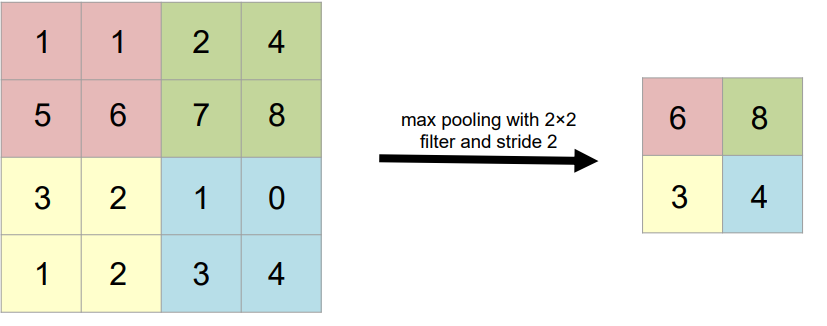
\includegraphics[scale = 0.5]{Pooling.PNG}

\end{figure}
Ele tá andando de 2 em 2 e pegando o maior valor, reduzindo a imagem. Então você aplica a convolução, usa a função de ativação depois disso e aí aplica o pooling, reduzindo tudo aos poucos e pegando o principal da imagem.

\subsubsection{Camada Final}
Em geral, a gente pega a camada final e achata ela como um vetorzão só, similar ao que fazíamos nas redes anteriores. Essa camada será similar às redes anteriores também no número de conexões, sendo totalmente conectada com a camada de outputs! Isso permite que tenhamos combinações não lineares das características de alto nível sendo 'aprendidas' para a classificação!

\subsection{Treinando CNNs}

\subsubsection{Funções de Ativação}
Nós sabemos que as redes neurais podem executar funções de ativação de alta complexidade. Por este motivo, entender o processo de backpropagation para o treinamento da rede pode acabar sendo complexo, e nos faz usar uma ferramenta de grafos computacionais.\par
Neles, pegamos todos os inputs da conta da rede, e vamos particionando a função em pequenas operações matemáticas, como soma, multiplicação, exponenciação, etc. Os inputs vão entrando e sendo 'transformados' até chegarmos ao resultado da função de ativação.
\newpage
Um exemplo de grafo computacional é o seguinte:
\begin{figure}[h]
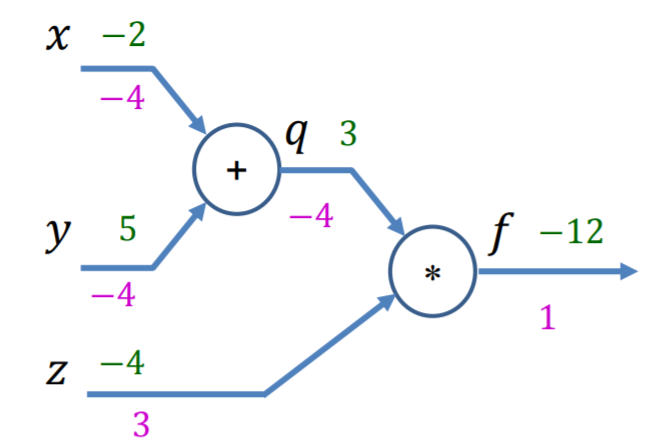
\includegraphics[scale = 0.4]{grafo.PNG}
\end{figure}
Em verde, vemos o que entra na operação do lado esquerdo e o que sai do lado direito. Vemos que a função é simples, dada por $f = z(x+y), q = x + y$. Em rosa, é a derivada relativa àquela variável. A derivada no ramo de baixo é, portanto $\frac{\partial f}{\partial z} = q = x + y$, e por aí vai. Meramente fazemos as contas da derivada de cada operação, e aí calculamos com os inputs, aplicando a regra da cadeia na ordem da direita pra esquerda! Por isso, é \textbf{back} propagation o negócio. Assim, a gente vai tendo um negócio menor e modularizado, que vai da esquerda pra direita pra calcular o resultado da função e da direita pra esquerda pra fazer o gradiente.\par
Existem uma série de possibilidades pras funções de ativação, e cada uma tem seus prós e contras. Como mencionado anteriormente, a sigmóide é útil, pois coloca os números na faixa de $[0,1]$. Só que tem alguns problemas:
a derivada da sigmóide é tal que, para valores muito extremos, ela é próxima de zero. Logo, o gradiente zera, e não adianta variar os pesos para o aprendizado ocorrer, pois os inputs vão ficar zerando o gradiente! \par
Além disso, a sigmóide não é centrada em zero. Isso significa que ela nunca assume valores negativos, e, portanto, os gradientes de todos os parâmetros vão sempre na mesma direção.
Logo, o que ocorre é que seu problema de aprendizado leva muito mais, porque os gradientes nos pesos ficam todos com o mesmo sinal, já que se todos os inputs do neurônio forem positivos, tudo vai sair positivo. Se o gradiente anterior vier negativo, sai negativo. Se vier positivo, sai positivo. Se o peso 'certo' for uma combinação de peso positivo com negativo, você vai ficar sempre andando em ziguezague.\par
Outra possibilidade é usar a função tanh(x) $ = \frac{e^x - e^{-x}}{e^x + e^{-x}}$. Ela só tem valores entre [-1,1], o que é bom, além de ser centrada em zero. Ainda assim, sua derivada tende a 0 para inputs extremos, o que mata o gradiente. \par
Uma função muito popular é a ReLU, que é simplesmente $\max(0,x)$. A derivada da ReLU é obviamente $1 \forall x \geq 0$. e 0 para todo resto. Isso significa que a derivada não vai para 0 para inputs positivos muito grandes. A função é extremamente rápida, mas tem seus problemas, já que ainda zera os gradientes com inputs negativos altos, além de não ser centrada em 0. A ReLU pode acabar 'morrendo', gerando um set de pesos tal que nenhum ponto dos seus dados tenha uma derivada não nula, e aí a ReLU dá o mesmo resultado para qualquer dado, e não temos bom aprendizado. \par
Aí uma forma boa de lidar com isso é uma LeakyReLU que é $\max(x) = (0.01x, x)$. A derivada é $0.01 \iff x < 0; 1 \iff x \geq 0$. Essa função nunca morre, não satura nunca, tem a média das ativações porra de zero e é bem eficiente, mas infelizmente não é centrada em zero. Podemos ter a PReLU, que faz $\max(x) = (\alpha x, x)$,que é bem parecida. \par
Por fim, falemos da ELU, que é $\alpha(e^x - 1) \forall x < 0; x, \forall x \geq 0$. Ela tem os mesmos benefícios da Leaky, mas satura em valores menores, e, portanto, é mais robusta à ruído. O problema é que não é centrada em zero. 
\subsubsection{Inicialização dos pesos}
Se usarmos pesos iniciais muito baixos, a propagação vai fazendo o gradiente desaparecer. Se usarmos pesos iniciais altos e tivermos funções que saturam nos extremos, o gradiente também irá desaparecendo na propagação! O tópico de qual o peso inicial ótimo ainda é um objeto de pesquisa interessante e em aberto, e vale se aprofundar na literatura para ter ideias do que usar. 
\subsubsection{Normalização}
Quando pegamos um dos minibatches previamente mencionados, podemos querer normalizar os dados por dimensão. Assim, tomamos um minibatch $m$, e, sob a dimensão $k$ desse minibatch, fazemos, para cada input i dessa dimensão, uma normalização:
\begin{gather*}
   \hat{x}_{m, k,i} = \frac{x_{m,k,i} - E[x_{m,k}]}{ \sqrt{Var[x_{m, k}]+\varepsilon}} 
\end{gather*}

Na ausência da média e do desvio-padrão teóricos, como de praxe usamos os dados empíricos \textbf{daquela} minibatch \textbf{naquela} dimensão. A constante $\varepsilon$ é apenas para estabilização numérica. \par
\subsubsection{Batch Normalizing Transform}
Pra sofisticar mais ainda, fazemos uma regressão: 
\begin{gather*}
    y_{m,k,i} = \gamma_k \hat{x_{m,k,i}} + \beta_k
\end{gather*}
Note que, se assim desejarmos, podemos usar os parâmetros $\gamma_k, \beta_k$ para reverter a normalização, caso isso faça sentido, bastando que $\gamma_k = \sqrt{Var[x_k]}, \beta_k = E[x_k]$. Os parâmetros também serão aprendidos pela rede, e, portanto, devem ser exclusivos das dimensões! \par
Mas qual o propósito desses parâmetros? Bem, primeiro que facilitamos o fluxo do gradiente. Segundo, reduzimos a dependência dos parâmetros de inicialização da rede e permitimos maiores taxas de aprendizado na rede, para que ela fique mais rápida sem que tenhamos tantos problemas. \par
Na hora de testar a rede, depois que ela foi adequadamente treinada, usamos a média e o desvio-padrão empírico previamente calculados! Não recalculamos estes valores para cada batch.
\subsection{}
\end{document}